\begin{center}
    \textbf{--------- Lezione 5 - 15 marzo 2021 ---------}
\end{center}

\subsubsection{Uso dei marcatori impliciti}
Data un'immagine, vogliamo capire dove ci troviamo rispetto ad essa. 
Gli ARUCO sono quadrilateri, invece un marcatore in un'immagine  non è detto che sia un quadrilatero, infatti può assumere diverse forme, come ad esempio una scatola di biscotti. 

Il riconoscimento di questi marker avviene con tecniche di template matching. 
Abbiamo due immagini: 
\begin{itemize}
    \item un template T: un'immagine di ciò che vogliamo riconoscere
    \item un'immagine C catturata con la camera
\end{itemize}
Vogliamo sapere se il template T compare nell'immagine C.
Serve il concetto di feature points.

I feature point sono piccole parti di un'immagine, tipicamente un insieme di pixel attorno ad un altro pixel. Ogni feature point è associato ad un feature descriptor. 
Scegliamo dei feature points che rimangono più o meno invariati anche se viene cambiata l'angolazione da cui si guarda.

Nell'esempio in figura \ref{fig:feature descriptor}, il feature descriptor sono i 16 pixel attorno.
\begin{figure}[!ht]
    \centering
    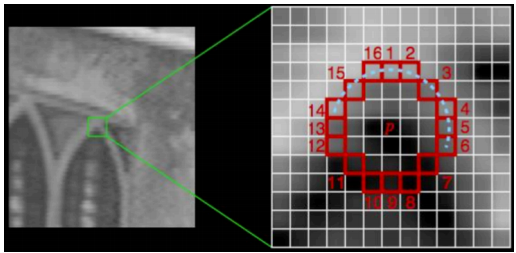
\includegraphics[width = .6\textwidth]{images/MobiDEV/3. augmented reality/feature points.PNG}
    \caption{}
    \label{fig:feature descriptor}
\end{figure}

Il pattern matching opera nel seguente modo: 
\begin{itemize}
    \item identifico il feature point nel template T e nell'immagine C presa dalla fotocamera
    \item trovo un modo per “far combaciare” (match) i feature points di T con quelli in C
    \item quando trovo il match corretto, se ho almeno 4 coppie di punti (4 in T e i corrispondenti 4 in C), posso calcolare l'omografia come per i marcatori espliciti. 
\end{itemize}

\begin{figure}[!ht]
    \centering
    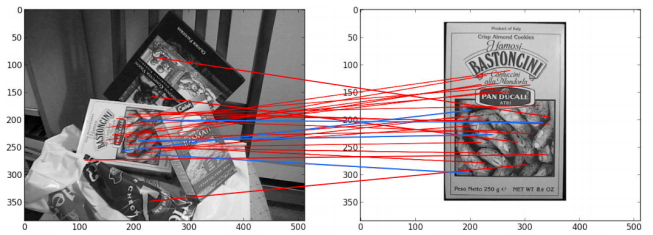
\includegraphics[width=\textwidth]{images/MobiDEV/3. augmented reality/pattern matching.PNG}
    \caption{}
    \label{fig:pattern matching}
\end{figure}

I feature points hanno un descriptor, dunque tipicamente cercherò di far combaciare due feature points (uno in T e l'altro in C) con descriptor simili, tuttavia potrebbero potrebbero esserci tanti feature points con descriptor simili, come in figura \ref{fig:pattern matching}. 

La prima tecnica è di provare tutte le combinazioni di punti, ma non funziona bene perché, anche se trovassi la combinazione giusta, avrei tante coppie il cui match non andrebbe bene. 
Quando trovo la combinazione giusta, basta qualche errore piccolo che non riesco a trovare la soluzione del sistema. 

Per risolvere il problema c'è RANSAC (Random sample Consensus): l'idea è di andare in modo casuale, ma in un modo simile agli ARUCO. 
Sceglie un'associazione casuale di 4 punti in T e C, e assumendo che queste 4 associazioni siano corrette, calcola l'omografia O. 
Usa O per verificare quanti altri punti combaciano.
Si ripete il procedimento fino a quando non si ottiene un certo livello minimo di punti che combaciano. 
L'algoritmo ha un aspetto in comune con quello usato per i marcatori espliciti: si ipotizza che una certa soluzione sia corretta e con quella si calcola l'omografia. Poi si usa quell'omografia per verificare se la soluzione è effettivamente corretta.

%Andiamo a togliere la dimensione prospettica solo dai fp in modo tale che posssiamo confrontare la posizione degli fp. 

\subsubsection{Registrazione visuale senza marcatori (markerless)}
In questo caso non abbiamo un'informazione predefinita da riconoscere, ma usiamo le caratteristiche dell'ambiente stesso per capire come ci stiamo spostando nell'ambiente.
Il problema è identificare in un'immagine i feature point di un oggetto non noto a priori non ci dice nulla sulla nostra posizione rispetto all'oggetto stesso. 
Ad esempio potremmo essere molto vicini ad un oggetto piccolo oppure molto lontani da un oggetto che appare identico, ma è grande e lontano.


Per avere dei sistemi di riferimento, usiamo due immagini e confrontiamo i feature points delle due immagini. Usiamo questi punti per capire come si rimappano tra di loro le due immagini.

Se le immagini invece sono prese da punti diversi nello spazio, prendo due immagini (o nello stesso istante se ho un dispositivo con fotocamere multiple, oppure 2 immagini a breve distanza) e uso la differenza prospettica per capire la distanza. 
\begin{figure}[!ht]
    \centering
    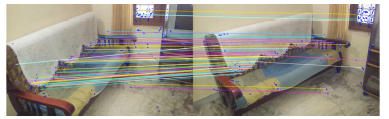
\includegraphics[width=\textwidth]{images/MobiDEV/3. augmented reality/markerless.PNG}
\end{figure}

\subsection{Il sistema di riferimento}
Quando facciamo la registration dobbiamo preoccuparsi che sistema di riferimento adottare: dove posizioniamo l'origine degli assi?
Questo dipende da cosa vogliamo fare:
\begin{itemize}
    \item alcuni sistemi adottano una registrazione su scala globale 
    \item in molti altri casi, è sufficiente un sistema di riferimento locale che tipicamente viene scelto in corrispondenza di un punto interessante (es: un marcatore o il volto dell'utente) o in un punto qualsiasi (es: nel punto in cui si trova il dispositivo quando viene fatta la prima registration)
\end{itemize}
